\subsection{Explicación del problema}

Dada una secuencia $A$ de números, se quieren pintar cada uno de ellos con rojo, azul o dejarlos sin pintar. 
 % Dicho de otro modo, cada número de la secuencia puede ser pintado de color rojo, azul o de ningun color. \\
Una aclaración importante es que los elementos de $A$ no pueden modificarse, ni tampoco cambiarse su orden inicial. Lo unico que puede hacerse con ellos es colorearlos (o no).\\

Para que una secuencia de colores se considere \textbf{válida} es necesario que se cumplan ciertas condiciones:
% Pintando $A$ de alguna forma se obtiene una secuencia de colores, pero no todas las secuencias de colores que pueden obtenerse son válidas.\\
% Decimos que una secuencia de colores es válida si se cumplen las siguientes condiciones:
\begin{enumerate}
\item Todos los elementos de color \textcolor{rojo}{rojo} están ordenados por valor de forma \underline{estrictamente creciente}
\item Todos los elementos de color \textcolor{azul}{azul} están ordenados por valor de forma \underline{estrictamente decreciente}
\end{enumerate}

\textit{(Estrictamente significa que no hay numeros consecutivos iguales)}\\

Las secuencias de colores válidas pueden tener diferentes cantidades de elementos sin pintar. \\
El objetivo del problema es encontrar la \textbf{mínima cantidad de elementos sin pintar} de todas las secuencias válidas que pueden formarse a partir de $A$. \\

% Más formalmente, sea $A$ una secuencia tal que \\

% {\centering 
%    $(\forall e \in A) ($ color($e$) $\in$ $\{$Rojo, Azul, Ninguno$\}$) \\
% }

\subsection{Ejemplo}

Supongamos que $A$ = [0, 7, 1, 2, 2, 1, 5, 0]. Veamos \textit{algunas} de las posibles secuencias de colores válidas: \\

{\centering 
  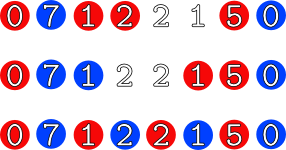
\includegraphics[width=0.50\textwidth]{informe/img/ejemplos/ejemplo1_finalsmall.png} \\
}

\vspace{1cm}
Consideremos los colores del tercer caso para ver que es una secuencia válida.
\begin{enumerate}
\item \textcolor{rojo}{\textbf{Rojos:}} [0, 1, 2, 5]  (estrictamente crecientes)
\item \textcolor{azul}{\textbf{Azules:}} [7, 2, 1, 0]  (estrictamente decrecientes)
\end{enumerate}

Podemos ver que diferentes formas de pintar de rojo y azul nos obligan a dejar algunos elementos sin pintar para que la secuencia sea válida. En el caso de este ejemplo la \textbf{mínima cantidad de elementos sin pintar} que puede obtenerse de $A$ es \textbf{0}, como puede verse en la tercer combinación. \\
